%%%%%%%%%%%%%%%%%%%%%%%%%%%%%%%%%%%%%%%%%%%%%%%%%%%%%%%%%%%%%%%%%%%%%%%%%%%%%%%%%%%%%%%%%%%%%%%%%%%%%%%%%%%%%%%%%%%%%%%%%%%%%%%%%%%%%%EJERCICIO 12 %%%%%%%%%%%%%%%%%%%%%%%%%%%%%%%%%%%%%%%%%%%%%%%%%%%%%%
    \textbf{Ejemplo 12}\\
	Se desean reunir 800.000 \ COP en 4 depósitos periódicos trimestre vencido crecientes en un 20\% más una cuota extra pactada de 80.000 \ COP en el período 2 trimestre vencido. Con una tasa del 20\% período trimestre vencido. Elabore la tabla de capitalización.\\
	 
	 \textbf{Solución 12}\\
	 %La tabla ira centrada
	 \begin{center}
	 	\renewcommand{\arraystretch}{1.5}% Margenes de las celdas
	 	%Creación de la cuadricula de 3 columnas
	 	\begin{longtable}[H]{|p{0.5\linewidth}|p{0.5\linewidth}|}
	 		%Creamos una linea horizontal
	 		\hline
	 		%Definimos el color de la primera fila
	 		\rowcolor[HTML]{FFB183}
	 		%%%%% INICIO ASIGNACIÓN período FOCAL %%%%%%%
	 		%%%%%%%%%% INICIO TITULO
	 		%Lo que se hace aquí es mezclar las 3 columnas en una sola
	 		\multicolumn{2}{|c|}{\cellcolor[HTML]{FFB183}\textbf{1. Asignación período focal}}   \\ \hline
	 		%%%%%%%%%% FIN TITULO
	 		%%%%% INICIO DECLARACIÓN DE VARIABLES %%%%%%%
	 		\multicolumn{2}{|c|}{$pf = 5 \textit{ ptv}$}\\ \hline
	 		%%%%%%%%%% INICIO TITULO
	 		%Lo que se hace aquí es mezclar las 3 columnas en una sola
	 		\multicolumn{2}{|c|}{\cellcolor[HTML]{FFB183}\textbf{2. Declaración de variables}}   \\ \hline
	 		%%%%%%%%%% FIN TITULO
	 		%%%%%%%%%% INICIO DE MATEMÁTICAS
	 		%Cada & hace referencia al paso de la siguiente columna
	 		$VF = 800.000 \ COP $  				& $ g = 20\%  $  \\
	 		$i = 20\%  \hspace{1mm} ptv$      	& $ R = 80.000 \ COP $ \\
	 		$n = 4 \hspace{1mm} ptv $           & $  $ \\ \hline
	 		%%%%%%%%%% FIN DE MATEMÁTICAS
	 		%%%%% FIN DECLARACIÓN DE VARIABLES
	 		
	 		\rowcolor[HTML]{FFB183}
	 		\multicolumn{2}{|c|}{\cellcolor[HTML]{FFB183}\textbf{3. Diagrama de flujo de caja}} \\ \hline
	 		\multicolumn{2}{|c|}{ 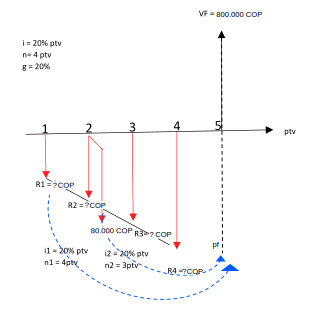
\includegraphics[trim=-78 -5 -78 -5]{7_Capitulo/img/ejemplos/12/12_1.pdf} }   \\ \hline
	 		%%%%% INICIO FLUJO DE CAJA
	 		\rowcolor[HTML]{FFB183}
	 		\multicolumn{2}{|c|}{\cellcolor[HTML]{FFB183}\textbf{4. Declaración de fórmulas}} \\ \hline
	 		%%%%%%%%%%%%% FIN INSERCIÓN DE IMAGEN
	 		%%%%%FIN FLUJO DE CAJA
	 		
	 		\multicolumn{2}{|c|}{ $VF = R n(1+i)^{n-1} $ Fórmula de Valor Futuro}   \\    \hline
	 		
	 		%%%%%% INICIO DESARROLLO MATEMÁTICO
	 		\rowcolor[HTML]{FFB183}
	 		%%%%%%%%%%INICIO TITULO
	 		\multicolumn{2}{|c|}{\cellcolor[HTML]{FFB183}\textbf{5. Desarrollo matemático}}       \\ \hline
	 		%%%%%%%%%% FIN TITULO
	 		%%%%%%%%%% INICIO MATEMÁTICAS
	 		\multicolumn{2}{|c|}{  $ 800.000 \ COP = R_{1} 4 ( 1 + 0,2)^{3} + 80.000 \ COP ( 1 + 0,2)^{2} $}   \\ 
	 		\multicolumn{2}{|c|}{  $  R_{1} = 99.074,07$ \ COP}  \\ 
	 		\multicolumn{2}{|c|}{  $  R_{2} = 99.074,07 \ COP ( 1 + 0,2)^{1} = 118.888,89 \ COP + 80.000 \ COP = 198.888,89 \ COP $}   \\ 
	 		\multicolumn{2}{|c|}{  $  R_{3} = 99.074,07 \ COP ( 1 + 0,2)^{2} = 142.666,67 \ COP $}   \\ 
	 		\multicolumn{2}{|c|}{ $  R_{4} = 99.074,07 \ COP ( 1 + 0,2)^{3}= 171.200,00 \ COP $}   \\  \hline
	 		
	 		%%%%%%%%%% FIN MATEMÁTICAS
	 		%%%%%% FIN DESARROLLO MATEMÁTICO
	 		%%%%%% INICIO RESPUESTA
	 		\rowcolor[HTML]{FFB183}
	 		%%%%%%%%%%INICIO TITULO
	 		\multicolumn{2}{|c|}{\cellcolor[HTML]{FFB183}\textbf{6. Respuesta}}   \\ \hline
	 		%%%%%%%%%% FIN TITULO
	 		%%%%%%%%%% INICIO RESPUESTA MATEMÁTICA
	 		\multicolumn{2}{|c|}{ 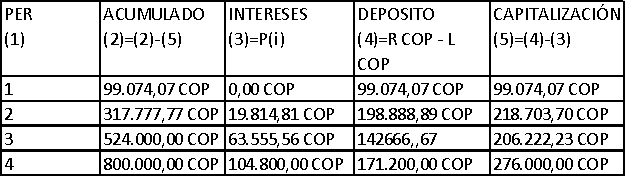
\includegraphics[trim=-78 -5 -78 -5]{7_Capitulo/img/ejemplos/12/12_2.pdf} }   \\ \hline
	 		%\multicolumn{2}{|C{\textwidth}|}{
	 		%	$R_{58} = 72.478,16 \ COP (1 + 0,02)^{57} = 224.087,15 \ COP $ 
	 		%}  \\ \hline
	 		
	 		
	 		%%%%%%%%%% FIN MATEMÁTICAS
	 		%%%%%% FIN RESPUESTA
	 	\end{longtable}
	 	%Se crean dos lineas en blanco para que no quede el siguiente texto tan pegado
	 	%\newline \newline %USARLO SI CREES QUE ES NECESARIO
	 \end{center}
  %%%%%%%%%%%%%%%%%%%%%%%%%%FIN EJERCICIO 12 %%%%%%%%%%%%%%%%%%%%%%%%%%%%%%%%%%%%%%%%%%%%%%%%%%%%%%%%%%%%%%%%%%%%%%%%%%%%%%%%%%%%%%%%%%%%%%%%%%%%%%%%%%%%